\BourbakiExercisesSection

\begin{enumerate}
\def\labelenumi{\arabic{enumi}.}
\item
  Let E, F be two A-modules and \(u: \mathbf{E} \to \mathbf{F}\) a linear mapping. Let M be a submodule of E, N a submodule of F, \(i: \mathbf{M} \to \mathbf{E}\) the canonical injection and \(q: \mathbf{F} \to \mathbf{F} / \mathbf{N}\) the canonical surjection. Show that \(u(\mathbf{M}) = \operatorname{Im}(u \circ i)\) and \(u^{-1}(\mathbf{N}) = \operatorname{Ker}(q \circ u)\) .
\item
  Let E be a left A-module; for every left ideal a of A let aE denote the sum of the ax where \(x \in E\) , which is therefore a submodule of E.
\end{enumerate}

\begin{enumerate}
\def\labelenumi{(\alph{enumi})}
\item
  Show that for every family \((\mathbf{E}_{\lambda})_{\lambda \in L}\) of A-modules, a. \(\bigoplus_{\lambda \in L} \mathbf{E}_{\lambda}\) is canonically identified with \(\bigoplus_{\lambda \in L} a E_{\lambda}\) .
\item
  If \(\mathfrak{a}\) is a finitely generated left ideal of \(\mathbf{A}\) , show that for every family \((\mathbf{E}_{\lambda})_{\lambda \in L}\) of \(\mathbf{A}\) -modules, \(\mathfrak{a}\) . \(\prod_{\lambda \in L} \mathbf{E}_{\lambda}\) is canonically identified with \(\prod_{\lambda \in L} \mathfrak{a}\mathbf{E}_{\lambda}\) . Give an example where \(\mathfrak{a}\) is not finitely generated and the above property fails to hold (take \(\mathbf{A}\) commutative and all the \(\mathbf{E}_{\lambda}\) equal to \(\mathbf{A}\) ).
\end{enumerate}

*(c) Let K be a commutative field, A the ring K{[}X,Y{]} of polynomials in two indeterminates over K, m = AX and n = AY. If E is the quotient A-module of \(\mathbf{A}^2\) by the submodule of \(\mathbf{A}^2\) generated by \(\mathbf{Xe}_1 - \mathbf{Ye}_2\) (where \((e_1, e_2)\) is the canonical basis of \(\mathbf{A}^2\) ), show that \((m \cap n)E \neq (mE) \cap (nE)\) .*

\begin{enumerate}
\def\labelenumi{\arabic{enumi}.}
\setcounter{enumi}{2}
\tightlist
\item
  Let E be an A-module.
\end{enumerate}

\begin{enumerate}
\def\labelenumi{(\alph{enumi})}
\tightlist
\item
  Let \((\mathbf{L}_{\mu})_{\mu \in \mathbf{M}}\) be a family of right directed ordered sets and, for all \(\mu \in \mathbf{M}\) , let \((\mathrm{F}_{\lambda \mu})_{\lambda \in L_{\mu}}\) be an increasing family of submodules of \(\mathbf{E}\) . Show that
\end{enumerate}

\[
\bigcap_ {\mu \in \mathbf {M}} \left(\sum_ {\lambda \in L _ {\mu}} F _ {\lambda \mu}\right) = \sum_ {\rho \in \prod_ {\mu} L _ {\mu}} \left(\bigcap_ {\mu \in \mathbf {M}} F _ {\rho (\mu), \mu}\right).
\]

\begin{enumerate}
\def\labelenumi{(\alph{enumi})}
\setcounter{enumi}{1}
\tightlist
\item
  Take A to be a field and E the A-module \(A^{N}\) ; let G be the submodule \(\mathbf{A}^{(\mathbf{N})}\) of E; on the other hand, for every finite subset H of N, let \(F_{H}\) be the submodule \(\prod_{n\in \mathbf{N}}\mathbf{M}_n\) of \(\mathbf{E}\) , where \(\mathbf{M}_n = \mathbf{A}\) for \(n\notin \mathrm{H}\) and \(\mathbf{M}_n = 0\) for \(n\in \mathrm{H}\) . Show that the family \((\mathrm{F_H})\) , where \(\mathbf{H}\) runs throughout the set \(\Phi\) of finite subsets of \(\mathbf{N}\) is right directed and that
\end{enumerate}

\[
\left(\bigcap_ {\mathrm{H} \in \Phi} \mathrm{F} _ {\mathrm{H}}\right) + \mathrm{G} \neq \bigcap_ {\mathrm{H} \in \Phi} (\mathrm{F} _ {\mathrm{H}} + \mathrm{G}).
\]

\begin{enumerate}
\def\labelenumi{\arabic{enumi}.}
\setcounter{enumi}{3}
\tightlist
\item
  Let \(\mathbf{E}, \mathbf{F}_1, \mathbf{F}_2\) be three A-modules and \(f_1: \mathbf{F}_1 \to \mathbf{E}\) , \(f_2: \mathbf{F}_2 \to \mathbf{E}\) two A-linear mappings. The fibre product of \(\mathbf{F}_1\) and \(\mathbf{F}_2\) relative to \(f_1\) and \(f_2\) is the submodule of the product \(\mathbf{F}_1 \times \mathbf{F}_2\) consisting of the ordered pairs \((x_1, x_2)\) such that \(f_1(x_1) = f_2(x_2)\) ; it is denoted by \(\mathbf{F}_1 \times_{\mathbf{E}} \mathbf{F}_2\) .
\end{enumerate}

\begin{enumerate}
\def\labelenumi{(\alph{enumi})}
\item
  For every ordered pair of A-linear mappings \(u_1 \colon G \to F_1, u_2 \colon G \to F_2\) such that \(f_1 \circ u_1 = f_2 \circ u_2\) , there exists one and only one A-linear mapping \(u \colon G \to F_1 \times_E F_2\) such that \(p_1 \circ u = u_1, p_2 \circ u = u_2\) , where \(p_1\) and \(p_2\) denote the restrictions to \(F_1 \times_E F_2\) of the projections \(pr_1\) and \(pr_2\) .
\item
  Let \(\mathbf{E}'\) , \(\mathbf{F}_1'\) , \(\mathbf{F}_2'\) be three A-modules, \(f_1': \mathbf{F}_1' \to \mathbf{E}', f_2': \mathbf{F}_2' \to \mathbf{E}'\) A-linear mappings and \(\mathbf{F}_1' \times_{\mathbf{E}'} \mathbf{F}_2'\) the fibre product relative to these mappings. For every system of A-linear mappings \(v_1: \mathbf{F}_1 \to \mathbf{F}_1'\) , \(v_2: \mathbf{F}_2 \to \mathbf{F}_2'\) , \(w: \mathbf{E} \to \mathbf{E}'\) such that \(f_1' \circ v_1 = w \circ f_1, f_2' \circ v_2 = w \circ f_2\) , let \(v\) be the A-linear mapping of \(\mathbf{F}_1 \times_{\mathbf{E}} \mathbf{F}_2\) into \(\mathbf{F}_1' \times_{\mathbf{E}'} \mathbf{F}_2'\) corresponding to the two linear mappings \(v_1 \circ p_1\) and \(v_2 \circ p_2\) . Show that if \(v_1\) and \(v_2\) are injective, so is \(v\) ; give an example where \(v_1\) and \(v_2\) are surjective but \(v\) is not surjective (take \(\mathbf{E}' = \{0\}\) ). If \(w\) is injective and \(v_1\) and \(v_2\) surjective, show that \(v\) is surjective.
\end{enumerate}

\begin{enumerate}
\def\labelenumi{\arabic{enumi}.}
\setcounter{enumi}{4}
\tightlist
\item
  Let \(\mathbf{E}, \mathbf{F}_1, \mathbf{F}_2\) be three A-modules and \(f_1: \mathbf{E} \to \mathbf{F}_1, f_2: \mathbf{E} \to \mathbf{F}_2\) two linear mappings. The amalgamated sum of \(\mathbf{F}_1\) and \(\mathbf{F}_2\) relative to \(f_1\) and \(f_2\) is the quotient module of \(\mathbf{F}_1 \times \mathbf{F}_2\) by the submodule the image of \(\mathbf{E}\) under the mapping \(z \mapsto (f_1(z), -f_2(z))\) ; it is denoted by \(\mathbf{F}_1 \oplus_{\mathbf{E}} \mathbf{F}_2\) .
\end{enumerate}

\begin{enumerate}
\def\labelenumi{(\alph{enumi})}
\tightlist
\item
  For every ordered pair of A-linear mappings \(u_{1}: \mathbf{F}_{1} \to \mathbf{G}, u_{2}: \mathbf{F}_{2} \to \mathbf{G}\) such that \(u_{1} \circ f_{1} = u_{2} \circ f_{2}\) , show that there exists one and only one A-linear mapping \(u: \mathbf{F}_{1} \oplus_{\mathbf{E}} \mathbf{F}_{2} \to \mathbf{G}\) such that \(u \circ j_{1} = u_{1}, u \circ j_{2} = u_{2}\) , where \(j_{1}\) and \(j_{2}\) denote the respective compositions of the canonical mapping
\end{enumerate}

\[
\mathbf {F} _ {1} \times \mathbf {F} _ {2} \rightarrow \mathbf {F} _ {1} \oplus_ {\mathrm{E}} \mathbf {F} _ {2}
\]

with the canonical injections \(\mathbf{F}_1\to \mathbf{F}_1\times \mathbf{F}_2,\mathbf{F}_2\rightarrow \mathbf{F}_1\times \mathbf{F}_2.\)

\begin{enumerate}
\def\labelenumi{(\alph{enumi})}
\setcounter{enumi}{1}
\tightlist
\item
  Let \(\mathbf{E}'\) , \(\mathbf{F}_1'\) , \(\mathbf{F}_2'\) be three A-modules, \(f_1': \mathbf{E}' \to \mathbf{F}_1'\) , \(f_2': \mathbf{E}' \to \mathbf{F}_2'\) two A-linear mappings and \(\mathbf{F}_1' \oplus_{\mathbf{E}'} \mathbf{F}_2'\) the amalgamated sum relative to these mappings. For every system of A-linear mappings \(v_1: \mathbf{F}_1' \to \mathbf{F}_1\) , \(v_2: \mathbf{F}_2' \to \mathbf{F}_2\) , \(w: \mathbf{E}' \to \mathbf{E}\) such that \(v_1 \circ f_1' = f_1 \circ w\) , \(v_2 \circ f_2' = f_2 \circ w\) , let \(v\) be the A-linear mapping of \(\mathbf{F}_1' \oplus_{\mathbf{E}'} \mathbf{F}_2'\) into \(\mathbf{F}_1 \oplus_{\mathbf{E}} \mathbf{F}_2\) corresponding to the two linear mappings \(j_1 \circ v_1\) and \(j_2 \circ v_2\) . Show that if \(v_1\) and \(v_2\) are surjective, so is \(v\) ; give an example where \(v_1\) and \(v_2\) are injective but \(v\) is not injective. Show that if \(w\) is surjective and \(v_1\) and \(v_2\) injective, then \(v\) is injective.
\end{enumerate}

\begin{enumerate}
\def\labelenumi{\arabic{enumi}.}
\setcounter{enumi}{5}
\tightlist
\item
  Given an A-module E, let \(\gamma(E)\) denote the least of the cardinals of the generating systems of E.
\end{enumerate}

\begin{enumerate}
\def\labelenumi{(\alph{enumi})}
\tightlist
\item
  If \(0 \to \mathbf{E} \to \mathbf{F} \to \mathbf{G} \to 0\) is an exact sequence of A-modules, then
\end{enumerate}

\[
\gamma (\mathbf {G}) \leqslant \gamma (\mathbf {F}) \leqslant \gamma (\mathbf {E}) + \gamma (\mathbf {G}).
\]

Give an example of a product \(\mathbf{F} = \mathbf{E} \times \mathbf{G}\) such that \(\gamma(\mathbf{E}) = \gamma(\mathbf{F}) = \gamma(\mathbf{G}) = 1\) (take \(\mathbf{E}\) and \(\mathbf{G}\) to be quotients of \(\mathbf{Z}\) ).

\begin{enumerate}
\def\labelenumi{(\alph{enumi})}
\setcounter{enumi}{1}
\item
  If \(\mathbf{E}\) is the sum of a family \((\mathrm{F}_{\lambda})_{\lambda \in L}\) of submodules, then \(\gamma (\mathbf{E})\leqslant \sum_{\lambda \in L}\gamma (\mathbf{F}_{\lambda}).\)
\item
  If \(\mathbf{M}\) and \(\mathbf{N}\) are submodules of a module \(\mathbf{E}\) , show that
\end{enumerate}

\[
\sup (\gamma (\mathbf {M}), \gamma (\mathbf {N})) \leqslant \gamma (\mathbf {M} \cap \mathbf {N}) + \gamma (\mathbf {M} + \mathbf {N}).
\]

\begin{enumerate}
\def\labelenumi{\arabic{enumi}.}
\setcounter{enumi}{6}
\tightlist
\item
  \begin{enumerate}
  \def\labelenumii{(\alph{enumii})}
  \tightlist
  \item
    Let A be a ring and E an (A, A)-bimodule; on the product \(B = A \times E\) a ring structure is defined by setting
  \end{enumerate}
\end{enumerate}

\[
(a, x) (a ^ {\prime}, x ^ {\prime}) = (a a ^ {\prime}, a x ^ {\prime} + x a ^ {\prime});
\]

E (canonically identified with \(\{0\} \times \mathbf{E}\) ) is then a two-sided ideal of B such that \(\mathbf{E}^2 = \{0\}\) .

\begin{enumerate}
\def\labelenumi{(\alph{enumi})}
\setcounter{enumi}{1}
\tightlist
\item
  By suitably choosing A and E, show that E can be a left B-module with \(\gamma(\mathbf{E})\) (Exercise 6) an arbitrary cardinal, although \(\gamma(\mathbf{B}_{s}) = 1\) .
\end{enumerate}

*8. Let A be a commutative ring, \(\mathbf{B} = \mathbf{A}[\mathbf{X}_n]_{n\geqslant 1}\) a polynomial ring over A in an infinity of indeterminates and C the quotient ring of B by the ideal generated by the polynomials \((\mathbf{X}_1 - \mathbf{X}_2)\mathbf{X}_i\) for \(i\geqslant 3\) . If \(\xi_1\) and \(\xi_2\) are the classes in C of \(\mathbf{X}_1\) and \(\mathbf{X}_2\) respectively, show that the intersection in C of the monogenous ideals \(\mathrm{C}\xi_1\) and \(\mathrm{C}\xi_2\) is not a finitely generated ideal.*

\begin{enumerate}
\def\labelenumi{\arabic{enumi}.}
\setcounter{enumi}{8}
\item
  Show that in an A-module E, if \((\mathrm{F}_{n})_{n\geqslant1}\) is a strictly increasing sequence of finitely generated submodules, the submodule F of E the union of the \(F_{n}\) is not finitely generated. Deduce that if E is an A-module which is not finitely generated, there exists a submodule F of E such that \(\gamma(\mathrm{F})=\aleph_{0}(=\mathrm{Card}(\mathbf{N}))\) .
\item
  Let E be a Z-module the direct sum of two submodules M, N respectively isomorphic to Z/2Z and Z/3Z; show that there exists no other decomposition of E as a direct sum of two non-zero submodules.
\item
  Let A be a ring admitting a field of left fractions (I, § 9, Exercise 15). Show that in the A-module \(A_{s}\) , a submodule distinct from \(A_{s}\) and \(\{0\}\) admits no supplementary submodule (cf.~I, § 9, Exercise 16).
\item
  Let \(\mathbf{G}\) be a module and \(\mathbf{E}, \mathbf{F}\) two submodules such that \(\mathbf{E} \subset \mathbf{F}\) .
\end{enumerate}

\begin{enumerate}
\def\labelenumi{(\alph{enumi})}
\item
  If F is a direct factor of G, F/E is a direct factor of G/E. If also E is a direct factor of F, E is a direct factor of G.
\item
  If E is a direct factor of G, then E is a direct factor of F. If also F/E is a direct factor of G/E, then F is a direct factor in G.
\item
  Give an example of two submodules \(\mathbf{M}, \mathbf{N}\) of the \(\mathbf{Z}\) -module \(\mathbf{E} = \mathbf{Z}^2\) such that \(\mathbf{M}\) and \(\mathbf{N}\) are direct factors of \(\mathbf{E}\) but \(\mathbf{M} + \mathbf{N}\) is not a direct factor of \(\mathbf{E}\) .
\item
  Let \(p\) be a prime number and \(U_p\) the submodule of the \(\mathbf{Z}\) -module \(\mathbf{Q} / \mathbf{Z}\) consisting of the classes mod \(\mathbf{Z}\) of rational numbers of the form \(k / p^n\) ( \(k \in \mathbf{Z}\) , \(n \in \mathbf{N}\) ). Let \(E\) be the product \(\mathbf{Z}\) -module \(M \times N\) , where \(M\) and \(N\) are both isomorphic to \(U_p\) , \(M\) and \(N\) being canonically identified with submodules of \(E\) . Consider the endomorphism \(u: (x, y) \mapsto (x, y + px)\) of \(E\) ; show that \(u\) is bijective. If \(M' = u(M)\) , show that \(M\) and \(M'\) are both direct factors of \(E\) but that \(M \cap M'\) is not a direct factor of \(E\) (use (b), showing that the \(Z\) -module \(U_p\) has no direct factor other than itself and \{0\}).
\end{enumerate}

¶ 13. Let E be an A-module and B the ring End\_A E. Show that for an element \(u \in B\) the following three conditions are equivalent: (1) Bu is a direct factor of the left B-module B\_s; (2) uB is a direct factor of the right B-module B\_d; (3) Ker(u) and Im(u) are direct factors of the A-module E. (Observe that every left ideal which is a direct factor of B\_s is of the form Bp, where p is a projector in E; cf.~I, § 8, Exercise 12 and use II, § 1, no. 9, Corollaries 1 and 2 to Proposition 15.)

\begin{enumerate}
\def\labelenumi{\arabic{enumi}.}
\setcounter{enumi}{13}
\tightlist
\item
  Let L be a well-ordered set, E an A-module and \((\mathbf{E}_{\lambda})_{\lambda \in L}\) an increasing family of submodules of E such that: (1) there exists a \(\lambda \in L\) such that \(E_{\lambda} = \{0\}\) ; (2) E is the union of the \(E_{\lambda}\) for \(\lambda \in L\) ; (3) if \(\lambda \in L\) is such that the set of \(\mu < \lambda\) admits a greatest element \(\lambda'\) , \(E_{\lambda}\) is the direct sum \(E_{\lambda'}\) and a submodule \(F_{\lambda}\) ; (4) if \(\lambda \in L\) is the least upper bound of the set of \(\mu < \lambda\) , then \(E_{\lambda}\) is the union of the \(E_{\mu}\) for \(\mu < \lambda\) . Under these conditions, show that E is the direct sum of the \(F_{\lambda}\) . (Prove by transfinite induction that each \(E_{\lambda}\) is the direct sum of the \(F_{\mu}\) such that \(\mu \leqslant \lambda\) .)
\end{enumerate}

¶ 15. Let c be an infinite cardinal.

\begin{enumerate}
\def\labelenumi{(\alph{enumi})}
\item
  Let I be a set and \(R\{a, b\}\) a relation between elements of I such that for all \(\alpha \in I\) the set of \(\beta \in I\) for which \(R\{\alpha, \beta\}\) holds has cardinal \(\leqslant c\) . Show that there exists a well-ordered set L and an increasing family \((\mathrm{I}_{\lambda})_{\lambda \in L}\) of subsets of I such that: (1) there exists a \(\lambda \in L\) such that \(I_{\lambda} = \varnothing\) ; (2) I is the union of the \(I_{\lambda}\) for \(\lambda \in L\) ; (3) if \(\lambda \in L\) is such that the set of \(\mu < \lambda\) has a greatest element \(\lambda'\) , \(\text{Card}(\mathbf{I}_{\lambda} - \mathbf{I}_{\lambda'}) \leqslant c\) ; (4) if \(\lambda \in L\) is the least upper bound of the set of \(\mu < \lambda\) , \(I_{\lambda}\) is the union of the \(I_{\mu}\) for \(\mu < \lambda\) ; (5) if \(\alpha \in I_{\lambda}\) and \(R\{\alpha, \beta\}\) holds, then \(\beta \in I_{\lambda}\) . (Note first that for all \(\alpha \in I\) the set of \(\beta \in I\) for which there exists an integer n and a sequence \((\gamma_{j})_{1 \leqslant j \leqslant n}\) of elements of I such that \(\gamma_{1} = \alpha, \gamma_{n} = \beta\) and \(R\{\gamma_{j}, \gamma_{j+1}\}\) holds for \(1 \leqslant j \leqslant n - 1\) , has cardinal \(\leqslant c\) . Then construct the \(I_{\lambda}\) by transfinite induction.)
\item
  Let E be an A-module the direct sum of a family \((\mathbf{M}_{\alpha})_{\alpha\in I}\) of submodules such that \(\gamma(\mathbf{M}_{\alpha})\leqslant c\) for all \(\alpha\in I\) (cf.~Exercise 6). Let f be an endomorphism of E. Show that there exists a well-ordered set L and an increasing family \((\mathbf{I}_{\lambda})_{\lambda\in L}\) of subsets of I satisfying properties (1), (2), (3) and (4) of (a) and such moreover that if we write \(\mathbf{E}_{\lambda} = \bigoplus_{\alpha \in \mathbf{I}_{\lambda}} \mathbf{M}_{\alpha}\) , then \(f(\mathbf{E}_{\lambda}) \subset \mathbf{E}_{\lambda}\) . (Apply (a) to the relation \(R\{\alpha, \beta\}\) : ``there exists \(x \in \mathbf{M}_{\alpha}\) such that the component of \(f(x)\) in \(\mathbf{M}_{\beta}\) is \(\neq 0\)''.) For all \(\lambda \in \mathbf{L}\) such that the set of \(\mu < \lambda\) has a greatest element \(\lambda'\) , write \(\mathbf{F}_{\lambda} = \bigoplus_{\alpha \in \mathbf{I}_{\lambda} - \mathbf{I}_{\lambda'}} \mathbf{M}_{\alpha}\) . Show that \(\mathbf{E}\) is the direct sum of the \(\mathbf{F}_{\lambda}\) (apply Exercise 14).
\item
  With the hypotheses and notation of (b), suppose further that \(f\) is a projector and write \(\mathbf{P} = f(\mathbf{E})\) . Let \(\mathbf{P}_{\lambda} = \mathbf{P} \cap \mathbf{E}_{\lambda}\) ; show that if \(\lambda \in \mathbf{L}\) is such that the set of \(\mu < \lambda\) has a greatest element \(\lambda'\) , \(\mathbf{P}_{\lambda'}\) is a direct factor of \(\mathbf{P}_{\lambda}\) (cf.~Exercise 12), that a supplementary submodule \(\mathbf{P}_{\lambda}'\) of \(\mathbf{P}_{\lambda'}\) in \(\mathbf{P}_{\lambda}\) is isomorphic to a direct factor of \(\mathbf{F}_{\lambda}\) and that \(\gamma(\mathbf{P}_{\lambda}') \leqslant c\) . Show that \(\mathbf{P}\) is the direct sum of the \(\mathbf{P}_{\lambda}'\) (apply Exercise 14).
\item
  Deduce from (c) that if an A-module E is the direct sum of a family \((\mathrm{M}_{\alpha})_{\alpha\in I}\) of submodules such that \(\gamma(\mathrm{M}_{\alpha})\leqslant\mathfrak{c}\) , then every direct factor P of E is also the direct sum of a family \((\mathrm{N}_{\lambda})_{\lambda\in L}\) of submodules such that \(\gamma(\mathrm{N}_{\lambda})\leqslant\mathfrak{c}\) .
\end{enumerate}

\begin{enumerate}
\def\labelenumi{\arabic{enumi}.}
\setcounter{enumi}{15}
\tightlist
\item
  Let A be a ring such that there exists an A-module M with a generating system of n elements but containing a free system of \(n + 1\) elements.
\end{enumerate}

\begin{enumerate}
\def\labelenumi{(\alph{enumi})}
\item
  Show that there exists in \(\mathbf{A}_s^n\) a free system of \(n + 1\) elements.
\item
  Deduce that there exists in M an infinite free system (construct such a system by induction using (a)).
\item
  Let C be a ring, E the free C-module \(\mathrm{C}_{s}^{(\mathrm{N})}, (e_{n})\) its canonical basis and A the endomorphism ring of E. Let \(u_{1}\) and \(u_{2}\) denote the endomorphisms of E defined by the conditions \(u_{1}(e_{2n}) = e_{n}, u_{1}(e_{2n+1}) = 0, u_{2}(e_{2n+1}) = e_{n}, u_{2}(e_{2n}) = 0\) for all \(n \geqslant 0\) . Show that \(u_{1}\) and \(u_{2}\) form a basis of the A-module \(A_{s}\) and deduce that in the A-module \(A_{s}\) there exist infinite free systems.
\end{enumerate}

*(d) Let A be the tensor algebra of a vector space E of dimension \(\geqslant 2\) over a commutative field (cf.~III, § 5, no. 1). Show that in the A-module \(A_s\) there exist infinite free systems (observe that two linearly independent vectors in E are linearly independent in \(A_s\) and use \((b)\) ). On the other hand, for every integer \(n > 0\) , every basis of the A-module \(A_s^n\) has \(n\) elements (cf.~§ 7, no. 2, Proposition 3).*

\begin{enumerate}
\def\labelenumi{\arabic{enumi}.}
\setcounter{enumi}{16}
\tightlist
\item
  Let A be a ring.
\end{enumerate}

\begin{enumerate}
\def\labelenumi{(\alph{enumi})}
\item
  Show that if the A-module \(\mathbf{A}_s^n\) is isomorphic to no \(\mathbf{A}_s^m\) for \(m > n\) , then, for all \(p < n\) , \(\mathbf{A}_s^p\) is isomorphic to no \(\mathbf{A}_s^q\) for \(q > p\) .
\item
  Show that if the A-module \(A_{s}^{n}\) contains no free system of \(n + 1\) elements, the A-module \(A_{s}^{p}\) contains no free system of \(p + 1\) elements for p \textless{} n.
\end{enumerate}

\begin{enumerate}
\def\labelenumi{\arabic{enumi}.}
\setcounter{enumi}{17}
\tightlist
\item
  Let A be a ring for which there exists an integer \(p\) with the following property: for every family \((a_i)_{1 \leqslant i \leqslant p}\) of \(p\) elements of A, there exists a family \((c_i)_{1 \leqslant i \leqslant p}\) of elements of A, one at least of which is not a right divisor of 0, such that \(\sum_{i=1}^{p} c_i a_i = 0\) .
\end{enumerate}

\begin{enumerate}
\def\labelenumi{(\alph{enumi})}
\item
  Show, by induction on \(n\) , that for every family \((x_{i})\) of \(p^n\) elements of \(A_s^n\) , there exists a family \((c_j)\) of \(p^n\) elements of \(A\) , one at least of which is not a right divisor of 0, such that \(\sum_{j} c_j x_j = 0\) .
\item
  Deduce from (a) and Exercise 16 that for all n \textgreater{} 0, the A-module \(A_{s}^{n}\) contains no free system of \(n + 1\) elements.
\end{enumerate}

\begin{enumerate}
\def\labelenumi{\arabic{enumi}.}
\setcounter{enumi}{18}
\tightlist
\item
  Let A be a non-zero ring with no divisors of zero.
\end{enumerate}

\begin{enumerate}
\def\labelenumi{(\alph{enumi})}
\item
  Show that for \(n > 1\) , the A-module \(\mathbf{A}_s^n\) is not monogenous.
\item
  Given an integer \(n \geqslant 1\) , for the A-module \(\mathbf{A}_s^n\) to contain no free system of \(n + 1\) elements, it is necessary that A admit a field of left fractions (I, §9, Exercise 15); conversely, if this condition is satisfied, \(\mathbf{A}_s^n\) contains a free system of \(n + 1\) elements for no integer \(n > 0\) . (Use Exercises 17 and 18 and I, §9, Exercise 16.)
\item
  Show that if every left ideal of A is monogenous, A admits a field of left fractions (use (a) and I, § 9, Exercise 16).
\end{enumerate}

\begin{enumerate}
\def\labelenumi{\arabic{enumi}.}
\setcounter{enumi}{19}
\tightlist
\item
  \begin{enumerate}
  \def\labelenumii{(\alph{enumii})}
  \tightlist
  \item
    Let A be a ring admitting a field of left fractions (I, § 9, Exercise 15). Let E be an A-module; show that, if in E \((x_{i})_{1\leqslant i\leqslant r}\) is a free system and \(y,z\) two elements such that \(x_{1},\ldots ,x_{r},y\) on the one hand and \(x_{1},\ldots ,x_{r},z\) on the other are two related systems, then \(x_{2},\ldots ,x_{r},y,z\) is a related system.
  \end{enumerate}
\end{enumerate}

\begin{enumerate}
\def\labelenumi{(\alph{enumi})}
\setcounter{enumi}{1}
\tightlist
\item
  Let A be the quotient ring Z/6Z and let \((e_{1}, e_{2})\) be the canonical basis of \(A^{2}\) ; show that if \(a = 2e_{1} + 3e_{2}\) , a and \(e_{1}\) form a related system, as do a and \(e_{2}\) , although \(e_{1}\) and \(e_{2}\) form a free system.
\end{enumerate}

\begin{enumerate}
\def\labelenumi{\arabic{enumi}.}
\setcounter{enumi}{20}
\item
  Let A be a ring, b, c two elements of A which are not right divisors of 0, M the A-module A/Abc and N the submodule Ac/Abc of M. For N to be a direct factor in M, it is necessary and sufficient that there exist two elements x, y of A such that \(xb + cy = 1\) . (If \(\varepsilon\) is the class of 1 in M, show that a supplementary subspace of N in M is generated by an element of the form \((1 - yc)\varepsilon\) whose annihilator is the ideal Ac.)
\item
  If an A-module E admits a basis whose indexing set is I and one of the two sets A, I is infinite, show that E is equipotent to \(A \times I\) .
\item
  \begin{enumerate}
  \def\labelenumii{(\alph{enumii})}
  \tightlist
  \item
    Let M, N be two subsets of an A-module E and m and n their annihilators; show that the annihilator of M ∩ N contains m + n and give an example where it is distinct from m + n.
  \end{enumerate}
\end{enumerate}

\begin{enumerate}
\def\labelenumi{(\alph{enumi})}
\setcounter{enumi}{1}
\item
  In a product module \(\prod_{i} \mathbf{E}_{i}\) , the annihilator of a subset \(\mathbf{F}\) is the intersection of the annihilators of its projections.
\item
  In a free A-module, the annihilator of an element \(\neq0\) contains only left divisors of 0 in A; in particular, if A is a ring with no divisors of 0, every element \(\neq0\) of a free module is free.
\end{enumerate}

\begin{enumerate}
\def\labelenumi{\arabic{enumi}.}
\setcounter{enumi}{23}
\tightlist
\item
  Let E be an A-module and M, N two submodules of E. The transporter of M into N, denoted by N:M, is the set of \(a \in A\) such that \(aM \subset N\) ; it is a two-sided ideal of A, equal to \(\text{Ann}((\mathbf{M} + \mathbf{N})/\mathbf{N})\) .
\end{enumerate}

\begin{enumerate}
\def\labelenumi{(\alph{enumi})}
\item
  Let A be a commutative ring, M an A-module, N a sub-module of M and x an element of M; show that \(N \cap Ax = (N:Ax)x\) .
\item
  Let A be a commutative ring and \(a, b\) two ideals of A. Show that \(a:b \supset a\) and that \((a:b)/a\) is an A-module isomorphic to \(\operatorname{Hom}(A/b, A/a)\) .
\end{enumerate}

\begin{enumerate}
\def\labelenumi{\arabic{enumi}.}
\setcounter{enumi}{24}
\item
  Let E, F be two A-modules and \(u: E \to F\) a linear mapping. Show that the mapping \((x, y) \mapsto (x, y - u(x))\) of the product module \(E \times F\) to itself is an automorphism of \(E \times F\) . Deduce that if there exists a linear mapping \(v: F \to E\) and an \(a \in E\) such that \(v(u(a)) = a\) , there exists an automorphism w of \(E \times F\) such that \(w(a, 0) = (0, u(a))\) .
\item
  Let E be a free A-module with a basis containing at least two elements.
\end{enumerate}

\begin{enumerate}
\def\labelenumi{(\alph{enumi})}
\item
  Show that every semi-linear mapping of E into itself (relative to an automorphism of A) which permutes with all the automorphisms of E, is necessarily a homothety \(x \mapsto \alpha x (\alpha \in \mathbf{A})\) .
\item
  Deduce from (a) that the centre of \(\operatorname{End}_{\mathbf{A}}(\mathbf{E})\) is the ring of central homotheties, isomorphic to the centre of A.
\item
  Deduce from (a) that the centre of the group \(\mathbf{GL}(\mathbf{E})\) is the group of invertible central homotheties of E, which is isomorphic to the multiplicative group of invertible elements of the centre of A.
\end{enumerate}

\begin{enumerate}
\def\labelenumi{\arabic{enumi}.}
\setcounter{enumi}{26}
\tightlist
\item
  Let A be a commutative ring. Show that if an ideal \(\mathfrak{J}\) of A is a free A-module, then \(\mathfrak{J}\) is a monogenous A-module (in other words a principal ideal). Give an example showing that the proposition does not extend to the left ideals in a non-commutative ring (Exercise 16).
\end{enumerate}

\BourbakiExercisesSection

\begin{enumerate}
\def\labelenumi{\arabic{enumi}.}
\tightlist
\item
  \begin{enumerate}
  \def\labelenumii{(\alph{enumii})}
  \tightlist
  \item
    If A is a ring with no divisors of zero, show that every element \(\neq0\) of a projective A-module is free.
  \end{enumerate}
\end{enumerate}

\begin{enumerate}
\def\labelenumi{(\alph{enumi})}
\setcounter{enumi}{1}
\item
  Give an example of a projective A-module whose annihilator is non-zero (cf.~I, § 8, no. 11).
\item
  Show that the Z-module Q is not a projective Z-module. *(See Commutative Algebra, II, § 5, Exercise 11 for an example of a finitely generated projective module over an integral domain, which is not free.)*
\end{enumerate}

\begin{enumerate}
\def\labelenumi{\arabic{enumi}.}
\setcounter{enumi}{1}
\item
  Show that every projective A-module is the direct sum of a family of projective submodules each of which admits a countable number of generators (``Kaplansky's Theorem''; apply Exercise 15 of §1, to the case where E is a free module).
\item
  Let \(\mathfrak{c}\) be a cardinal and \(\mathbf{P}\) a projective A-module such that \(\gamma(\mathbf{P}) \leqslant \mathfrak{c}\) (§ 1,
\end{enumerate}

Exercise 6). Show that if L is a free A-module with an infinite basis of cardinal \(\geqslant c\) , P ⊕ L is isomorphic to L. (Observe that there exists a free A-module M, whose basis has cardinal \(\leqslant c\) , isomorphic to the direct sum of P and an A-module Q. Note that M \(^{(N)}\) and P ⊕ M \(^{(N)}\) are isomorphic.)

¶ 4. (a) Let E, E' be two A-modules, N a submodule of E and N' a submodule of E' such that E is projective and E/N and E'/N' are isomorphic. Show that there exists an exact sequence

\[
0 \longrightarrow \mathrm{N} \stackrel {u} {\longrightarrow} \mathrm{E} \oplus \mathrm{N} ^ {\prime} \stackrel {v} {\longrightarrow} \mathrm{E} ^ {\prime} \longrightarrow 0.
\]

(Observe that there exists a homomorphism \(f \colon \mathbf{E} \to \mathbf{E}'\) such that \(f(\mathbf{N}) \subset \mathbf{N}'\) , which gives when passing to the quotients an isomorphism \(\mathbf{E} / \mathbf{N} \to \mathbf{E}' / \mathbf{N}'\) ; define \(u\) and \(v\) in an analogous way to that used for the exact sequence (29) of §1, no. 7.)

\begin{enumerate}
\def\labelenumi{(\alph{enumi})}
\setcounter{enumi}{1}
\item
  Deduce from (a) that if \(\mathbf{E}'\) is projective, \(\mathbf{E} \oplus \mathbf{N}'\) and \(\mathbf{E}' \oplus \mathbf{N}\) are isomorphic.
\item
  Let \(0 \to \mathbf{E}_m \to \mathbf{E}_{m-1} \to \ldots \to \mathbf{E}_1 \to \mathbf{E}_0 \to 0\) be an exact sequence of A-modules such that \(\mathbf{E}_0, \mathbf{E}_1, \ldots, \mathbf{E}_{m-2}\) are projective. Show that the A-modules \(\bigoplus_{h \geqslant 0} \mathbf{E}_{m-2h}\) and \(\bigoplus_{h \geqslant 0} \mathbf{E}_{m-2h+1}\) are isomorphic (with the convention that \(\mathbf{E}_i = \{0\}\) for \(i < 0\) ).
\end{enumerate}

\begin{enumerate}
\def\labelenumi{\arabic{enumi}.}
\setcounter{enumi}{4}
\item
  Let \(u\) be a linear mapping from an A-module \(\mathbf{E}\) to an A-module \(\mathbf{F}\) and \(v = {}^t u\) its transpose. For every submodule \(\mathbf{N}'\) of \(\mathbf{F}^*\) , the submodule of \(\mathbf{E}\) orthogonal to \(v(\mathbf{N}')\) is \(\overline{u}^{-1}(\mathbf{N})\) , where \(\mathbf{N}\) is the submodule of \(\mathbf{F}\) orthogonal to \(\mathbf{N}'\) .
\item
  \begin{enumerate}
  \def\labelenumii{(\alph{enumii})}
  \tightlist
  \item
    If E is an A-module, every injective endomorphism u of E is not a left divisor of zero in the ring \(\operatorname{End}_{\mathbf{A}}(\mathbf{E})\) . Conversely, if for every sub-A-module \(F \neq \{0\}\) of E there exists an endomorphism \(v \neq 0\) of E such that \(v(\mathbf{E}) \subset \mathbf{F}\) , an element which is not a left divisor of zero in \(\operatorname{End}_{\mathbf{A}}(\mathbf{E})\) is an injective endomorphism. The above condition is satisfied if there exists a linear form \(x' \in E^*\) and an \(x \in E\) such that \(\langle x, x' \rangle\) is invertible in A and in particular if E is free.
  \end{enumerate}
\end{enumerate}

\begin{enumerate}
\def\labelenumi{(\alph{enumi})}
\setcounter{enumi}{1}
\item
  Every endomorphism \(\neq 0\) of the \(\mathbf{Z}\) -module \(\mathbf{Q}\) is bijective, although there exists no linear form \(\neq 0\) on \(\mathbf{Q}\) .
\item
  Let \(U_{p}\) be the Z-module defined in §1, Exercise 12(d). Show that the endomorphism \(x \mapsto px\) of \(U_{p}\) is not injective and is not a left divisor of zero in \(\operatorname{End}_{\mathbf{Z}}(\mathbf{U}_{p})\) .
\end{enumerate}

\begin{enumerate}
\def\labelenumi{\arabic{enumi}.}
\setcounter{enumi}{6}
\tightlist
\item
  \begin{enumerate}
  \def\labelenumii{(\alph{enumii})}
  \tightlist
  \item
    If \(u\) is a surjective endomorphism of an A-module \(\mathbf{E}\) , \(u\) is not a right divisor of zero in \(\operatorname{End}_{\mathbf{A}}(\mathbf{E})\) . Conversely, if for every submodule \(\mathbf{F} \neq \mathbf{E}\) of \(\mathbf{E}\) there exists a linear form \(x^{*} \in \mathbf{E}^{*}\) which is zero on \(\mathbf{F}\) and surjective, every element of \(\operatorname{End}_{\mathbf{A}}(\mathbf{E})\) which is not a right divisor of zero is a surjective endomorphism.
  \end{enumerate}
\end{enumerate}

\begin{enumerate}
\def\labelenumi{(\alph{enumi})}
\setcounter{enumi}{1}
\item
  If E is the Z-module defined in Exercise 6(c), show that every endomorphism \(\neq 0\) of E is surjective, although there exists no linear form \(\neq 0\) on E.
\item
  Show that if E is a free Z-module \(\neq0\) , there exist non-surjective endomorphisms of E which are not right divisors of 0 in \(\operatorname{End}_{\mathbf{Z}}(\mathbf{E})\) .
\end{enumerate}

\begin{enumerate}
\def\labelenumi{\arabic{enumi}.}
\setcounter{enumi}{7}
\tightlist
\item
  \begin{enumerate}
  \def\labelenumii{(\alph{enumii})}
  \tightlist
  \item
    Let E be a free A-module, F, G two A-modules and \(u: \mathbf{E} \to \mathbf{G}\) , \(v: \mathbf{F} \to \mathbf{G}\) two linear mappings. Show that if \(u(\mathbf{E}) \subset v(\mathbf{F})\) , there exists a linear mapping \(w: \mathbf{E} \to \mathbf{F}\) such that \(u = v \circ w\) .
  \end{enumerate}
\end{enumerate}

\begin{enumerate}
\def\labelenumi{(\alph{enumi})}
\setcounter{enumi}{1}
\item
  Give an example of two non-zero endomorphisms \(u, v\) of the \(\mathbf{Z}\) -module \(\mathbf{E}\) defined in Exercise 6(c) such that there exists no endomorphism \(w\) of \(\mathbf{E}\) for which \(u = v \circ w\) (although \(u(\mathbf{E}) = v(\mathbf{E}) = \mathbf{E}\) ).
\item
  Give an example of two endomorphisms \(u, v\) of the \(\mathbf{Z}\) -module \(\mathbf{Z}\) such that \(u^{-1}(0) = v^{-1}(0) = \{0\}\) , but such that there exists no endomorphism \(w\) of \(\mathbf{Z}\) for which \(u = w \circ v\) (cf.~§ 7, Exercise 14).
\end{enumerate}

\begin{enumerate}
\def\labelenumi{\arabic{enumi}.}
\setcounter{enumi}{8}
\tightlist
\item
  Given an A-module E, for every submodule M of E (resp. every submodule M' of E*), let M° (resp. M'°) denote the orthogonal of M in E* (resp. the orthogonal of M' in E). Consider the following four properties:
\end{enumerate}

\begin{enumerate}
\def\labelenumi{(\Alph{enumi})}
\item
  The canonical homomorphism \(c_{\mathbf{E}}: \mathbf{E} \to \mathbf{E}^{**}\) is bijective.
\item
  For every submodule M of E, the canonical homomorphism \(E^{*}/M^{\circ} \rightarrow M^{*}\) is bijective.
\item
  For every submodule M of E, \(M^{\circ\circ} = M\) .
\item
  For every ordered pair of submodules M, N of E,
\end{enumerate}

\[
(\mathbf {M} \cap \mathbf {N}) ^ {\circ} = \mathbf {M} ^ {\circ} + \mathbf {N} ^ {\circ}.
\]

\begin{enumerate}
\def\labelenumi{(\alph{enumi})}
\item
  Show that condition (B) implies (D) (prove that for \(x^{*} \in (\mathbf{M} \cap \mathbf{N})^{\circ}\) , there exists \(y^{*} \in \mathbf{E}^{*}\) such that \(\langle x + y, y^{*} \rangle = \langle x, x^{*} \rangle\) for \(x \in \mathbf{M}\) and \(y \in \mathbf{N}\) ).
\item
  Let A be a ring with no divisors of zero, but having no field of left fractions \(*\) (for example the tensor algebra of a vector space of dimension \textgreater1, cf.~III, § 5, Exercise 5) \(^{*}\) . If we take \(E = A_{s}\) , condition (A) is satisfied, but none of conditions (B), (C), (D) (for an example where (B), (C), (D) hold, but not (A), see § 7, no. 5, Theorem 6).
\item
  Take A to be a product ring \(\mathbf{K}^{\mathrm{I}}\) , where \(\mathbf{K}\) is a commutative field and I an infinite set. Show that the A-module \(\mathbf{E} = \mathbf{A}\) satisfies conditions (A) and (B), but not (C) (observe that the annihilators of the ideals of \(\mathbf{A}\) are all of the form \(\mathbf{K}^{\mathrm{J}}\) , where \(\mathbf{J} \subset \mathbf{I}\) ).
\item
  Suppose that for two submodules \(\mathbf{M},\mathbf{N}\) of \(\mathbf{E}\) such that \(\mathbf{N} \subset \mathbf{M}\) and \(\mathbf{N} \neq \mathbf{M}\) , the dual \((\mathbf{M} / \mathbf{N})^*\) is non-zero; then show that condition (B) implies (C).
\item
  The kernel of \(c_{\mathbf{E}}\) is the orthogonal \((\mathbf{E}^{*})^{\circ}\) of \(\mathbf{E}^{*}\) in \(\mathbf{E}\) . Give an example where neither \(\mathbf{E}^{*}\) nor \((\mathbf{E}^{*})^{\circ}\) is 0 (consider a module containing an element whose annihilator contains an element which is not a divisor of 0).
\item
  Let \(\mathbf{M}\) be a direct factor of \(\mathbf{E}\) ; show that \(\mathbf{M}^{\circ \circ} = \mathbf{M} + (\mathbf{E}^{*})^{\circ}\) .
\end{enumerate}

\begin{enumerate}
\def\labelenumi{\arabic{enumi}.}
\setcounter{enumi}{9}
\tightlist
\item
  Give an example of an A-linear mapping \(u: \mathbf{E} \to \mathbf{F}\) such that \(^t u\) is bijective but \(u\) is neither injective nor surjective (cf.~Exercise 6(b) and (c)).
\end{enumerate}

Deduce an example where \(y_{0} \in F\) is orthogonal to the kernel of \(^{t}u\) but where the equation \(u(x) = y_{0}\) has no solution.

¶ 11. Let A be a ring and I an A-module. I is called injective if, for every exact sequence \(\mathrm{E}' \to \mathrm{E} \to \mathrm{E}''\) of A-linear mappings, the sequence

\[
\operatorname{Hom} \left(\mathrm{E} ^ {\prime \prime}, \mathrm{I}\right)\rightarrow \operatorname{Hom} (\mathrm{E}, \mathrm{I}) \rightarrow \operatorname{Hom} \left(\mathrm{E} ^ {\prime}, \mathrm{I}\right)
\]

is exact.

\begin{enumerate}
\def\labelenumi{(\alph{enumi})}
\tightlist
\item
  Show that the following properties are equivalent:
\end{enumerate}

\((\alpha)\) I is injective.

(β) For every exact sequence \(0 \rightarrow E' \rightarrow E \rightarrow E'' \rightarrow 0\) of A-linear mappings, the sequence

\[
0 \rightarrow \operatorname{Hom} (\mathrm{E} ^ {\prime \prime}, \mathrm{I}) \rightarrow \operatorname{Hom} (\mathrm{E}, \mathrm{I}) \rightarrow \operatorname{Hom} (\mathrm{E} ^ {\prime}, \mathrm{I}) \rightarrow 0
\]

is exact.

(γ) For every A-module M and every submodule N of M, every A-linear mapping of N into I can be extended to an A-linear mapping of M into I.

(δ) For every left ideal \(\mathfrak{a}\) of A and every A-linear mapping \(f: \mathfrak{a} \to \mathbf{I}\) , there exists an element \(b \in \mathbf{I}\) such that \(f(a) = ab\) for all \(a \in \mathfrak{a}\) .

(ζ) I is a direct factor of every A-module containing it.

(θ) For every A-module E which is the sum of I and a monogenous submodule, I is a direct factor of E.

(To prove that (δ) implies (γ), show that property (δ) implies that if E is an A-module and F a submodule of E such that E/F is monogenous, then every linear mapping of F into I can be extended to a linear mapping of E into I. Then use Zorn's Lemma. To prove that (θ) implies (δ), consider the A-module \(A_{s} \times I = M\) , the submodule N of M consisting of the elements \((a, -f(a))\) for \(a \in \mathfrak{a}\) , and apply (θ) to the quotient module M/N.)

\begin{enumerate}
\def\labelenumi{(\alph{enumi})}
\setcounter{enumi}{1}
\tightlist
\item
  For a Z-module E to be injective, it is necessary and sufficient that for all \(x \in E\) and every integer \(n \neq 0\) , there exists \(y \in E\) such that ny = x. In particular, the Z-modules Q and Q/Z are injective.
\end{enumerate}

\begin{enumerate}
\def\labelenumi{\arabic{enumi}.}
\setcounter{enumi}{11}
\tightlist
\item
  \begin{enumerate}
  \def\labelenumii{(\alph{enumii})}
  \tightlist
  \item
    For a product \(\prod_{\lambda \in L} E_{\lambda}\) of A-modules to be injective (Exercise 11), it is necessary and sufficient that each of the \(E_{\lambda}\) be injective.
  \end{enumerate}
\end{enumerate}

\begin{enumerate}
\def\labelenumi{(\alph{enumi})}
\setcounter{enumi}{1}
\tightlist
\item
  Let K be a commutative field, L an infinite set and A the product ring \(K^{L}\) . Show that A is an injective A-module (use (a)) but that the ideal \(\mathfrak{a}\) of A the direct sum of the factors of \(K^{L}\) (canonically identified with ideals of A) is not an injective A-module.
\end{enumerate}

¶ 13. (a) Let A be a ring and I an injective A-module (Exercise 11) such that for every non-zero monogenous A-module E, there exists a non-zero A-homomorphism of E into I. Let M be an A-module, N a submodule of M and \(\tilde{\mathbf{N}}\) the set of \(u \in \operatorname{Hom}_{\mathbf{A}}(\mathbf{M}, \mathbf{I})\) such that \(u(x) = 0\) in N. Show that for all \(y \notin N\) , there exists a \(u \in \tilde{\mathbf{N}}\) such that \(u(y) \neq 0\) .

\begin{enumerate}
\def\labelenumi{(\alph{enumi})}
\setcounter{enumi}{1}
\item
  Let A be a ring. For every (A, A)-bimodule T and every left (resp. right) A-module M, \(\operatorname{Hom}_{\mathbf{A}}(\mathbf{M}, \mathbf{T})\) has canonically a right (resp. left) A-module structure deriving from that on T, and there is a canonical A-homomorphism \(c_{M,T}: M \to \operatorname{Hom}_{\mathbf{A}}(\operatorname{Hom}_{\mathbf{A}}(\mathbf{M}, \mathbf{T}), \mathbf{T})\) such that \(c_{M,T}(x)\) is the A-homomorphism \(u \mapsto u(x)\) . Show that if I is an (A, A)-bimodule which, as a left A-module, satisfies the conditions of (a), then the canonical homomorphism \(c_{M,I}\) is injective for every left A-module M.
\item
  Suppose that I is an (A, A)-bimodule which is injective as a left A-module and a right A-module and that for every (left or right) monogenous A-module \(E \neq 0\) , there exists a non-zero A-homomorphism of E into I. Show that under these conditions, if P is a left (resp. right) projective A-module, \(\operatorname{Hom}_{\mathbf{A}}(\mathbf{P}, \mathbf{I})\) is a right (resp. left) injective A-module. (Suppose that P is a left projective A-module. Observe that for every submodule \(N'\) of a right A-module N, \(\operatorname{Hom}_{\mathbf{A}}(\mathbf{N}', \mathbf{I})\) is isomorphic to a quotient module of \(\operatorname{Hom}_{\mathbf{A}}(\mathbf{N}, \mathbf{I})\) and apply (b) to the right module N and the left module P.)
\item
  Let C be a commutative ring, A a C-algebra and I an injective C-module such that for every monogenous C-module \(E \neq \{0\}\) there exists a non-zero C-homomorphism of E into I. For every A-module M, \(\operatorname{Hom}_{\mathbf{C}}(\mathbf{M}, \mathbf{I})\) is an A-module; show that for every projective A-module P, \(\operatorname{Hom}_{\mathbf{C}}(\mathbf{P}, \mathbf{I})\) is an injective A-module (same argument as in (c)).
\end{enumerate}

\begin{enumerate}
\def\labelenumi{\arabic{enumi}.}
\setcounter{enumi}{13}
\tightlist
\item
  Let A be a ring. Show that for every A-module M there exists an injective A-module I such that M is isomorphic to a submodule of I. (Apply Exercise 13(d) with C = Z, using Exercise 11(b) and the fact that every A-module is the quotient of a free A-module.)
\end{enumerate}

¶ 15. An A-module homomorphism \(u: \mathbf{E} \to \mathbf{F}\) is called essential if it is injective and if, for every submodule \(\mathbf{P} \neq \{0\}\) of \(\mathbf{F}\) , \(u^{-1}(\mathbf{P}) \neq \{0\}\) ; it suffices that this condition holds for every monogenous submodule \(\mathbf{P} \neq \{0\}\) of \(\mathbf{F}\) . If \(\mathbf{E}\) is a submodule of \(\mathbf{F}\) , \(\mathbf{F}\) is called an essential extension of \(\mathbf{E}\) if the canonical injection \(\mathbf{E} \to \mathbf{F}\) is essential.

\begin{enumerate}
\def\labelenumi{(\alph{enumi})}
\item
  Let \(u: \mathbf{E} \to \mathbf{F}\) , \(v: \mathbf{F} \to \mathbf{G}\) be two A-homomorphisms of A-modules. If \(u\) and \(v\) are essential, so is \(v \circ u\) . Conversely, if \(v \circ u\) is essential and \(v\) is injective, then \(u\) and \(v\) are essential.
\item
  Let E be a submodule of an A-module F and let \((\mathbf{F}_{\lambda})_{\lambda \in L}\) be a family of submodules of F containing E and whose union is F. Show that if each of the \(F_{\lambda}\) is an essential extension of E, so is F.
\item
  Let \((u_{\lambda})_{\lambda \in L}\) be a family of essential homomorphisms \(u_{\lambda} \colon \mathbf{E}_{\lambda} \to \mathbf{F}_{\lambda}\) . Show that the homomorphism \(\bigoplus_{\lambda \in L} u_{\lambda} \colon \bigoplus_{\lambda \in L} \mathbf{E}_{\lambda} \to \bigoplus_{\lambda \in L} \mathbf{F}_{\lambda}\) is essential. (Prove it first when \(L\) has two elements, then use (b).)
\item
  The \(\mathbf{Z}\) -module \(\mathbf{Q}\) is an essential extension of \(\mathbf{Z}\) but the product \(\mathbf{Q}^{\mathrm{N}}\) is not an essential extension of \(\mathbf{Z}^{\mathrm{N}}\) .
\item
  Let E be a submodule of a module F. Show that there exists a submodule
\end{enumerate}

Q of F such that \(Q \cap E = \{0\}\) and that the restriction to E of the canonical homomorphism \(F \to F/Q\) is essential.

\begin{enumerate}
\def\labelenumi{\arabic{enumi}.}
\setcounter{enumi}{15}
\tightlist
\item
  A submodule E of an A-module F is called irreducible with respect to F (or in F) if \(E \neq F\) and E is not the intersection of two submodules of F distinct from E.
\end{enumerate}

\begin{enumerate}
\def\labelenumi{(\alph{enumi})}
\item
  For an A-module F to be an essential extension of each of its submodules \(\neq \{0\}\) it is necessary and sufficient that \(\{0\}\) be irreducible with respect to F.
\item
  Let \((\mathbf{E}_{\lambda})_{\lambda \in L}\) be a family of submodules of an A-module \(\mathbf{F}\) . \((\mathbf{E}_{\lambda})_{\lambda \in L}\) is called a reduced irreducible decomposition of \(\{0\}\) in \(\mathbf{F}\) if each of the \(\mathbf{F}_{\lambda}\) is irreducible in \(\mathbf{F}\) , if the intersection of the \(\mathbf{E}_{\lambda}\) reduces to 0 and if none of the \(\mathbf{E}_{\lambda}\) contains the intersection of the \(\mathbf{E}_{\mu}\) for \(\mu \neq \lambda\) . When this is so, show that the canonical homomorphism of \(\mathbf{F}\) into \(\bigoplus_{\lambda \in L} (\mathbf{F} / \mathbf{E}_{\lambda})\) is essential (if \(\mathbf{E}_{\lambda}' = \bigcap_{\mu \neq \lambda} \mathbf{E}_{\mu}\) , observe that the image \(\mathbf{F}_{\lambda}'\) of \(\mathbf{E}_{\lambda}'\) in \(\mathbf{F} / \mathbf{E}_{\lambda}\) is non-zero and that the image of \(\mathbf{F}\) in \(\bigoplus_{\lambda \in L} (\mathbf{F} / \mathbf{E}_{\lambda})\) contains \(\bigoplus_{\lambda \in L} \mathbf{F}_{\lambda}'\) ; then apply Exercise 15(c)). Conversely, if \((\mathbf{E}_{\lambda})_{\lambda \in L}\) is a family of submodules of \(\mathbf{F}\) irreducible in \(\mathbf{F}\) and the canonical homomorphism \(\mathbf{F} \to \bigoplus_{\lambda \in L} (\mathbf{F} / \mathbf{E}_{\lambda})\) is essential, the family \((\mathbf{E}_{\lambda})\) is a reduced irreducible decomposition of \(\{0\}\) in \(\mathbf{F}\) .
\end{enumerate}

¶ 17. (a) Let M, N, M', N' be four submodules of a module E such that M ∩ N = M' ∩ N' = P. Show that

\[
\mathbf {M} = (\mathbf {M} + (\mathbf {N} \cap \mathbf {M} ^ {\prime})) \cap (\mathbf {M} + (\mathbf {N} \cap \mathbf {N} ^ {\prime})).
\]

Deduce that if \(\mathbf{M}\) is irreducible in \(\mathbf{E}\) , then necessarily \(\mathbf{P} = \mathbf{M}' \cap \mathbf{N}\) or \(\mathbf{P} = \mathbf{N}' \cap \mathbf{N}\) .

\begin{enumerate}
\def\labelenumi{(\alph{enumi})}
\setcounter{enumi}{1}
\tightlist
\item
  Let \((\mathrm{N}_{i})_{1\leqslant i\leqslant n}\) be a finite family of submodules of E irreducible in E and M its intersection. Show that if \((\mathrm{P}_{j})_{1\leqslant j\leqslant m}\) is a finite family of submodules of E such that \(M=\bigcap_{j}P_{j}\) , then for every index i such that \(1\leqslant i\leqslant n\) there exists an index \(\phi(i)\) such that \(1\leqslant\phi(i)\leqslant m\) and such that, if we write \(N_{i}^{\prime}=\bigcap_{k\neq i}N_{k}\) , then \(M=P_{\phi(i)}\cap N_{i}^{\prime}\) (use (a)). Deduce that if none of the \(P_{j}\) contains the intersection of the \(P_{k}\) of index \(\neq j\) , then \(m\leqslant n\) (successively replace the \(N_{i}\) by suitable \(P_{j}\) , using the above result). Conclude that two reduced irreducible decompositions of M in E, one of which is finite, necessarily have the same number of terms (cf.~Exercise 23).
\end{enumerate}

¶ 18. (a) For an A-module I to be injective, show that it is necessary and sufficient that I admit no essential extension distinct from itself (show that this condition implies condition (δ) of Exercise 11(a), arguing as for the proof that (θ) implies (δ) in that exercise).

\begin{enumerate}
\def\labelenumi{(\alph{enumi})}
\setcounter{enumi}{1}
\item
  Let I be an injective A-module. For a submodule E of I to be injective, it is necessary and sufficient that E admit no essential extension distinct from itself and contained in I (using Exercise 15(e)), show that this condition implies that E is a direct factor of I).
\item
  Let I be an injective A-module, E a submodule of I and \(h: \mathbf{E} \to \mathbf{F}\) an essential homomorphism. Show that there exists an injective homomorphism \(j: \mathbf{F} \to \mathbf{I}\) such that \(j \circ h\) is the canonical injection of E into I.
\item
  Let I be an A-module and E a submodule of I. Show that the following properties are equivalent:
\end{enumerate}

(α) I is injective and is an essential extension of E.

(β) I is injective and for every injective homomorphism \(j\) of \(E\) into an injective A-module \(J\) , there exists an injective homomorphism of \(I\) into \(J\) extending \(j\) .

(γ) I is injective and is the smallest injective submodule of I containing E.

(δ) I is an essential extension of E and for every essential homomorphism \(h: E \to F\) , there exists an injective homomorphism \(j: F \to I\) such that \(j \circ h\) is the canonical injection of E into I.

(Use (c) and (a).) When these equivalent conditions hold, I is called an injective envelope of E; I is then also an injective envelope of every submodule of I containing E.

\begin{enumerate}
\def\labelenumi{(\alph{enumi})}
\setcounter{enumi}{4}
\item
  Let I be an injective A-module and E a submodule of I. Show that every maximal element of the set of essential extensions of E contained in I is an injective envelope of E (use (b)). In particular, every A-module admits an injective envelope (cf.~Exercise 14).
\item
  If I, I' are two injective envelopes of the same A-module E, show that there exists an isomorphism of I onto I' leaving invariant the elements of E.
\end{enumerate}

¶ 19. (a) Let E, F be two A-modules and M an injective submodule of E ⊕ F. Let I be an injective envelope of M ∩ E in M and J a supplementary submodule of I in M. Show that the restriction to I (resp. J) of the canonical projection of E ⊕ F onto E (resp. F) is injective (compose with the projection of I into E an extension E → I of the injection M ∩ E → I).

\begin{enumerate}
\def\labelenumi{(\alph{enumi})}
\setcounter{enumi}{1}
\tightlist
\item
  Let E be an A-module and M a submodule of E, maximal in the set of injective submodules of E; M admits in E a supplementary submodule N which contains no injective submodule \(\neq\{0\}\) . Show that for every injective submodule P of E, the image of P under the projection of E onto M (under the decomposition of E as a direct sum \(M \oplus N\) ) is an injective envelope of \(P \cap M\) in M (use (a)). If \(M'\) is another submodule of E which is maximal in the set of injective submodules of E, show that there exists an automorphism of E transforming M into \(M'\) and leaving invariant the elements of N.
\end{enumerate}

¶ 20. (a) Let A be a ring admitting a field of left fractions K (I, § 9, Exercise 15). Show that K, considered as a left A-module, is an injective envelope of A \(_{s}\) . (Apply criterion (α) of Exercise 18(d) and criterion (δ) of Exercise 11(a) noting that if f: a → K is an A-linear mapping of a left ideal a of A into K, the element \(x^{-1}f(x)\) for \(x \in \mathfrak{a}, x \neq 0\) (the inverse being taken in K) does not depend on \(x \in \mathfrak{a}\) .)

\begin{enumerate}
\def\labelenumi{(\alph{enumi})}
\setcounter{enumi}{1}
\tightlist
\item
  Let \(U_{p}\) be the sub-Z-module of Q/Z consisting of the canonical images of the rational numbers of the form \(k/p^{n}\) , where p is a given prime number, \(k \in Z\) and \(n \in N\) (II, §1, Exercise 12(d)). Show that \(U_{p}\) is an injective envelope of each of the Z-modules \(p^{-n}Z/Z\) isomorphic to \(Z/p^{n}Z\) . Show that there exist automorphisms of \(U_{p}\) distinct from the identity automorphism leaving invariant the elements of a submodule \(p^{-n}Z/Z\) .
\end{enumerate}

¶ 21. (a) Let \((\mathbf{E}_j)_{j \in J}\) be a finite family of A-modules and for all \(j \in J\) let \(I_j\) be an injective envelope of \(E_j\) ; show that \(\bigoplus_{j \in J} I_j\) is an injective envelope of \(\bigoplus_{j \in J} E_j\) .

\begin{enumerate}
\def\labelenumi{(\alph{enumi})}
\setcounter{enumi}{1}
\tightlist
\item
  An A-module M is called indecomposable if it is distinct from \(\{0\}\) and it is not the direct sum of two submodules distinct from \(\{0\}\) . Show that if I is an injective A-module, the following properties are equivalent:
\end{enumerate}

\((\alpha)\) \(\{0\}\) is an irreducible submodule in I.

(β) I is indecomposable.

(γ) I is an injective envelope of each of its submodules \(\neq0\) . (Use (a) and Exercise 18 (e).)

(δ) I is isomorphic to the injective envelope \(\mathrm{I}(\mathrm{A}/\mathrm{q})\) , where q is an irreducible left ideal of A.

Moreover, when this is so, for all \(x \neq 0\) in I, \(\operatorname{Ann}(x)\) is an irreducible left ideal of A and I is isomorphic to \(\operatorname{I}(\mathbf{A} / \operatorname{Ann}(x))\) .

Deduce that for the injective envelope of an A-module E to be indecomposable, it is necessary and sufficient that \(\{0\}\) be an irreducible submodule of E.

\begin{enumerate}
\def\labelenumi{(\alph{enumi})}
\setcounter{enumi}{2}
\item
  Give an example of an indecomposable Z-module E such that its injective envelope I(E) is decomposable (cf.~VII, § 3, Exercise 5).
\item
  Let E be an A-module, I an injective envelope of E and \(I = \bigoplus_{\lambda \in L} I_{\lambda}\) a decomposition of I as a direct sum of a finite family of indecomposable injective submodules; for all \(\lambda \in L\) let \(J_{\lambda} = \bigoplus_{\mu \neq \lambda} I_{\mu}\) and let \(N_{\lambda} = J_{\lambda} \cap E\) . Show that \((\mathrm{N}_{\lambda})_{\lambda \in L}\) is a reduced irreducible decomposition of \(\{0\}\) in E (Exercise 16 (b)) and that \(I_{\lambda}\) is an injective envelope of \(E/N_{\lambda}\) . Conversely, every reduced irreducible decomposition of \(\{0\}\) in E can be obtained by the above procedure uniquely up to isomorphism (use Exercise 16 (b)).
\end{enumerate}

\begin{enumerate}
\def\labelenumi{\arabic{enumi}.}
\setcounter{enumi}{21}
\tightlist
\item
  Let I be an injective A-module. If I is indecomposable, every injective endomorphism of I is an automorphism of I. Deduce that, for I to be indecomposable, it is necessary and sufficient that the non-invertible elements of the ring End(I) form a two-sided ideal of that ring.
\end{enumerate}

¶ 23. Let M be an A-module, the direct sum of a family (finite or otherwise) \((\mathbf{M}_{\lambda})_{\lambda \in L}\) of submodules such that for all \(\lambda \in L\) the non-invertible elements of \(\operatorname{End}(\mathbf{M}_{\lambda})\) form a two-sided ideal of this ring (which implies that \(\mathbf{M}_{\lambda}\) is indecomposable).

\begin{enumerate}
\def\labelenumi{(\alph{enumi})}
\item
  Let \(f, g\) be two endomorphisms of \(\mathbf{M}\) such that \(f + g = 1_{\mathbf{M}}\) . Show that for every finite sequence \((\lambda_k)_{1 \leqslant k \leqslant s}\) of distinct indices in \(\mathbf{L}\) there exists a family of submodules \(\mathbf{N}_k\) ( \(1 \leqslant k \leqslant s\) ) of \(\mathbf{M}\) such that for every \(k\) one of the endomorphisms \(f, g\) restricted to \(\mathbf{M}_{\lambda_{k}}\) is an isomorphism of this submodule onto \(\mathbf{N}_k\) and that \(\mathbf{M}\) is the direct sum of the \(\mathbf{N}_k\) ( \(1 \leqslant k \leqslant s\) ) and the \(\mathbf{M}_{\lambda}\) for \(\lambda\) distinct from \(\lambda_k\) . (Reduce it to the case \(s = 1\) ; if \(\pi_{\lambda}\) is the canonical projection of \(\mathbf{M}\) onto \(\mathbf{M}_{\lambda}\) corresponding to the decomposition as a direct sum of \(\mathbf{M}_{\lambda}\) and \(\bigoplus_{\mu \neq \lambda} \mathbf{M}_{\mu}\) , note that either \(\pi_{\lambda} \circ f\) or \(\pi_{\lambda} \circ g\) , restricted to \(\mathbf{M}_{\lambda}\) , is an automorphism of \(\mathbf{M}_{\lambda}\) .)
\item
  Let \(f\) be an idempotent endomorphism of \(\mathbf{M}\) . Show that there exists at least one index \(\lambda \in \mathbf{L}\) such that the restriction of \(f\) to \(\mathbf{M}_{\lambda}\) is an isomorphism of \(\mathbf{M}_{\lambda}\) onto \(f(\mathbf{M}_{\lambda})\) ; moreover \(f(\mathbf{M}_{\lambda})\) is a direct factor of \(\mathbf{M}\) . (If \(g = 1_{\mathbf{M}} - f\) , note that there exists a finite sequence of indices \((\lambda_k)_{1 \leqslant k \leqslant s}\) such that the intersection of \(\operatorname{Ker}(g)\) and the direct sum of the \(\mathbf{M}_{\lambda_k}\) is \(\neq \{0\}\) and use (a).)
\item
  Deduce from (b) that every indecomposable direct factor of M is isomorphic to one of the \(M_{\lambda}\) .
\item
  Let \((\mathrm{N}_{\kappa})_{\kappa\in K}\) be a family of indecomposable submodules of M of which M is the direct sum; every \(N_{\kappa}\) is therefore isomorphic to an \(M_{\lambda}\) and vice versa, by virtue of (c). Let T be the set of classes of indecomposable submodules of M (under the relation of isomorphism) such that an \(M_{\lambda}\) (or an \(N_{\kappa}\) ) belongs to one of these classes. For all \(t\in T\) , let \(\mathrm{R}(t)\) (resp. \(\mathrm{S}(t)\) ) be the set of \(\lambda\in L\) (resp. \(\kappa\in K\) ) such that \(M_{\lambda}\in t\) (resp. \(N_{\kappa}\in t\) ). Show that, for all \(t\in T\) , \(\mathrm{Card}(\mathrm{R}(t))=\mathrm{Card}(\mathrm{S}(t))\) . (In the notation of (a), let \(\mathrm{J}(\kappa)\) be the set of \(\lambda\in L\) such that the restriction of \(\pi_{\lambda}\) to \(N_{\kappa}\) is an isomorphism of \(N_{\kappa}\) onto \(M_{\lambda}\) ; show that \(\mathrm{J}(\kappa)\) is finite and that the \(\mathrm{J}(\kappa)\) cover \(\mathrm{R}(t)\) when \(\kappa\) runs through \(\mathrm{S}(t)\) . Deduce that \(\mathrm{Card}(\mathrm{S}(t))\leqslant\mathrm{Card}(\mathrm{R}(t))\) when \(\mathrm{R}(t)\) is infinite. When \(\mathrm{R}(t)\) is finite, show with the aid of (a) that M is the direct sum of the \(M_{\lambda}\) for \(\lambda\notin R(t)\) and a subfamily of \((\mathrm{N}_{\kappa})_{\kappa\in\mathrm{S}(t)}\) of cardinal equal to that of \(\mathrm{R}(t)\) .
\item
  Deduce from (d) and Exercises 22 and 21 (d) that if \((\mathbf{E}_{\lambda})_{\lambda \in L}\) and \((\mathbf{E}_{\kappa}^{\prime})_{\kappa \in K}\) are two reduced irreducible decompositions of \(\{0\}\) in a module F, L and K are equipotent.
\end{enumerate}

\begin{enumerate}
\def\labelenumi{\arabic{enumi}.}
\setcounter{enumi}{23}
\item
  Let M be an A-module, I its injective envelope (Exercise 18), \(\mathfrak{a}\) a two-sided ideal of A and Q the submodule of I consisting of the \(z \in I\) such that \(\mathfrak{a}z = \{0\}\) ; Q has a natural \((\mathrm{A}/\mathfrak{a})\) -module structure. Let N be the submodule of M consisting of the \(x \in M\) such that \(\mathfrak{a}x = \{0\}\) ; if N is considered as an \((\mathrm{A}/\mathfrak{a})\) -module, show that Q is isomorphic to an injective envelope of N.
\item
  \begin{enumerate}
  \def\labelenumii{(\alph{enumii})}
  \tightlist
  \item
    For an A-module \(\mathbf{Q}\) to be injective, it is sufficient that, for every projective A-module P and every submodule \(P'\) of P, every linear mapping of \(P'\) into Q can be extended to a linear mapping of P into Q (use the fact that every A-module is a quotient of a projective A-module).
  \end{enumerate}
\end{enumerate}

\begin{enumerate}
\def\labelenumi{(\alph{enumi})}
\setcounter{enumi}{1}
\tightlist
\item
  For an A-module P to be projective, it is sufficient that, for every injective A-module Q and every quotient module \(Q''\) of Q, every homomorphism of P into \(Q''\) be of the form \(\phi \circ u\) , where \(\phi: Q \to Q''\) is the canonical homomorphism and u is a homomorphism of P into Q (use the fact that every A-module is a submodule of an injective A-module).
\end{enumerate}

\begin{enumerate}
\def\labelenumi{\arabic{enumi}.}
\setcounter{enumi}{25}
\tightlist
\item
  For every Z-module G and every integer n \textgreater{} 0, let \(_{n}G\) denote the kernel of the endomorphism \(x \mapsto nx\) of G. If \(0 \to G' \to G \to G'' \to 0\) is an exact sequence, define a canonical homomorphism \(d:_{n}G'' \to G'/nG'\) such that the sequence
\end{enumerate}

\[
0 \longrightarrow_ {n} G ^ {\prime} \longrightarrow_ {n} G ^ {\prime \prime} \stackrel {d} {\longrightarrow} G ^ {\prime} / n G ^ {\prime} \longrightarrow G / n G \longrightarrow G ^ {\prime \prime} / n G ^ {\prime \prime} \longrightarrow 0
\]

is exact. If \(_n\mathrm{G}\) and \(\mathrm{G} / n\mathrm{G}\) are finite, we write

\[
h _ {n} (\mathrm{G}) = \operatorname{Card} (\mathrm{G} / n \mathrm{G}) - \operatorname{Card} (_ {n} \mathrm{G});
\]

then show that \(_{n}G'\) , \(_{n}G''\) , \(G'/nG'\) , \(G''/nG''\) are finite and that

\[
h _ {n} (\mathrm{G}) = h _ {n} \left(\mathrm{G} ^ {\prime}\right) + h _ {n} \left(\mathrm{G} ^ {\prime \prime}\right).
\]

\BourbakiExercisesSection

\begin{enumerate}
\def\labelenumi{\arabic{enumi}.}
\tightlist
\item
  Let A be a ring, E a right A-module and F a left A-module. Let f be a function defined on the set S of all finite sequences
\end{enumerate}

\[
((x _ {1}, y _ {1}), (x _ {2}, y _ {2}), \dots , (x _ {n}, y _ {n})) \quad (n \text {   arbitrary })
\]

of elements of \(\mathbf{E} \times \mathbf{F}\) with values in a set \(\mathbf{G}\) and such that:

\[
f ((x _ {1}, y _ {1}), \dots , (x _ {n}, y _ {n})) = f ((x _ {\sigma (1)}, y _ {\sigma (1)}), \dots , (x _ {\sigma (n)}, y _ {\sigma (n)}))\tag{1}
\]

for every permutation \(\sigma \in \mathfrak{S}_n\) ;

\[
\begin{array}{r l} f \left(\left(x _ {1} + x _ {1} ^ {\prime}, y _ {1}\right), \left(x _ {2}, y _ {2}\right), \dots , \left(x _ {n}, y _ {n}\right)\right) & = f \left(\left(x _ {1}, y _ {1}\right), \left(x _ {1} ^ {\prime}, y _ {1}\right), \left(x _ {2}, y _ {2}\right), \dots , \left(x _ {n}, y _ {n}\right)\right); \end{array} \tag {2}
\]

\[
f ((x _ {1}, y _ {1} + y _ {1} ^ {\prime}), (x _ {2}, y _ {2}), \dots , (x _ {n}, y _ {n})) = f ((x _ {1}, y _ {1}), (x _ {1}, y _ {1} ^ {\prime}), (x _ {2}, y _ {2}), \dots , (x _ {n}, y _ {n}));\tag{3}
\]

\[
f ((x _ {1} \lambda , y _ {1}), \dots , (x _ {n}, y _ {n})) = f ((x _ {1}, \lambda y _ {1}), \dots , (x _ {n}, y _ {n}))\tag{4}
\]

for all \(\lambda \in \mathbf{A}\) .

Show that there exists one and only one mapping \(g\) of \(\mathbf{E} \otimes_{\mathbf{A}} \mathbf{F}\) into \(\mathbf{G}\) such that \(f((x_1, y_1), \ldots, (x_n, y_n)) = g\left(\sum_{i=1}^{n} x_i \otimes y_i\right)\) . (Note that if

\[
\sum_ {i} x _ {i} \otimes y _ {i} = \sum_ {j} x _ {j} ^ {\prime} \otimes y _ {j} ^ {\prime},
\]

the difference \(\sum_{i}(x_i, y_i) - \sum_j(x'_j, y'_j)\) in the \(\mathbf{Z}\) -module \(\mathbf{Z}^{(\mathbf{E} \times \mathbf{F})}\) is a linear combination with integer coefficients of elements of the form (2) of no. 1.)

*2. Consider the field \(\mathbf{C}\) of complex numbers as a vector space over the field \(\mathbf{R}\) of real numbers.

\begin{enumerate}
\def\labelenumi{(\alph{enumi})}
\item
  Show that the canonical mapping \(\mathbf{C} \otimes_{\mathbf{R}} \mathbf{C} \to \mathbf{C} \otimes_{\mathbf{C}} \mathbf{C}\) is not injective.
\item
  Show that the two \(\mathbf{C}\) -module structures on \(\mathbf{C} \otimes_{\mathbf{R}} \mathbf{C}\) arising from each of the factors are distinct*.
\end{enumerate}

\begin{enumerate}
\def\labelenumi{\arabic{enumi}.}
\setcounter{enumi}{2}
\tightlist
\item
  \begin{enumerate}
  \def\labelenumii{(\alph{enumii})}
  \tightlist
  \item
    Let \((\mathbf{E}_{\lambda})_{\lambda \in L}\) be a family of right A-modules and F a left A-module. Show that if F is finitely generated, the canonical mapping
  \end{enumerate}
\end{enumerate}

\[
\left(\prod_ {\lambda \in L} E _ {\lambda}\right) \otimes_ {A} F \rightarrow \prod_ {\lambda \in L} (E _ {\lambda} \otimes_ {A} F)
\]

is surjective.

\begin{enumerate}
\def\labelenumi{(\alph{enumi})}
\setcounter{enumi}{1}
\item
  Give an example of a commutative ring A and an ideal m of A such that the canonical mapping \(\mathbf{A}^{\mathbf{N}}\otimes_{\mathbf{A}}(\mathbf{A}/\mathfrak{m})\to(\mathbf{A}/\mathfrak{m})^{\mathbf{N}}\) is not injective (cf.~§1, Exercise 2 (b)).
\item
  Give an example of a commutative ring A such that the canonical mapping \(A^{N} \otimes_{A} A^{N} \to A^{N \times N}\) is not surjective (observe that for given n, the
\end{enumerate}

image of \(\mathbf{N}\) under a mapping of the form \(m \mapsto \sum_{i=1}^{n} u_i(m)v_i(n)\) , where the \(u_i\) and \(v_i\) belong to \(\mathbf{A}^{\mathbf{N}}\) , generate a finitely generated ideal of \(\mathbf{A}\) .

\begin{enumerate}
\def\labelenumi{(\alph{enumi})}
\setcounter{enumi}{3}
\tightlist
\item
  Deduce from (b) and (c) an example where the canonical homomorphism (22) (no. 7) is neither injective nor surjective.
\end{enumerate}

\begin{enumerate}
\def\labelenumi{\arabic{enumi}.}
\setcounter{enumi}{3}
\tightlist
\item
  Let E be a right A-module and F a free left A-module. Show that if x is a free element of E and y an element \(\neq0\) of F, then \(x\otimes y\neq0\) ; if also A is commutative and y is a free element of F, then \(x\otimes y\) is free in the A-module \(E\otimes_{A}F\) .
\end{enumerate}

\BourbakiExercisesSection

\begin{enumerate}
\def\labelenumi{\arabic{enumi}.}
\tightlist
\item
  Let A, B be two rings, E a left A-module, F a right A-module and G an (A, B)-bimodule; \(\operatorname{Hom}_{\mathbf{B}}(\mathbf{F}, \mathbf{G})\) then has a left A-module structure and \(\operatorname{Hom}_{\mathbf{A}}(\mathbf{E}, \mathbf{G})\) a right B-module structure. Show that the Z-modules
\end{enumerate}

\[
\operatorname{Hom} _ {\mathbf {A}} (\mathrm{E}, \operatorname{Hom} _ {\mathbf {B}} (\mathrm{F}, \mathrm{G})) \quad \text { and } \quad \operatorname{Hom} _ {\mathbf {B}} (\mathrm{F}, \operatorname{Hom} _ {\mathbf {A}} (\mathrm{E}, \mathrm{G}))
\]

are both canonically isomorphic to the Z-module of Z-bilinear mappings f of \(E \times F\) into G such that \(f(\alpha x, y) = \alpha f(x, y)\) and \(f(x, y\beta) = f(x, y)\beta\) for \(\alpha \in A\) , \(\beta \in B\) , \(x \in E\) , \(y \in F\) .

\begin{enumerate}
\def\labelenumi{\arabic{enumi}.}
\setcounter{enumi}{1}
\tightlist
\item
  Let A be the ring Z/4Z, m the ideal 2Z/4Z of A and E the A-module
\end{enumerate}

A/m. Show that the canonical mapping \(E^{*} \otimes_{A} E \to \operatorname{Hom}_{A}(E, E)\) is neither injective nor surjective. The same is true of the canonical mapping

\[
\mathbf {E} \otimes_ {\mathbf {A}} \mathbf {E} \rightarrow \operatorname{Hom} _ {\mathbf {A}} (\mathbf {E} ^ {*}, \mathbf {E})
\]

and the canonical mapping \(\mathbf{E}^{*}\otimes_{\mathbf{A}}\mathbf{E}^{*}\to (\mathbf{E}\otimes_{\mathbf{A}}\mathbf{E})^{*}\) .

\begin{enumerate}
\def\labelenumi{\arabic{enumi}.}
\setcounter{enumi}{2}
\item
  Show that under the conditions of no. 2, if E is assumed to be a finitely generated left A-module and F a projective right B-module, the canonical homomorphism (7) (no. 2) is bijective.
\item
  Given an example where the canonical homomorphism (21) (no. 4) is neither injective nor surjective, although \(F_{2} = C\) , \(E_{1} = C\) and \(E_{2}\) and \(F_{1}\) are finitely generated C-modules (cf.~Exercise 2).
\item
  Let A, B be two rings, E a right A-module, F a left A-module and G a (B, A)-bimodule.
\end{enumerate}

\begin{enumerate}
\def\labelenumi{(\alph{enumi})}
\tightlist
\item
  Show that there exists one and only one Z-linear mapping
\end{enumerate}

\[
\eta : \mathrm{E} \otimes_ {\mathrm{A}} \mathrm{F} \rightarrow \operatorname{Hom} _ {\mathrm{B}} (\operatorname{Hom} _ {\mathrm{A}} (\mathrm{E}, \mathrm{G}), \mathrm{G} \otimes_ {\mathrm{A}} \mathrm{F})
\]

which maps the tensor product \(x \otimes y\) , where \(x \in \mathbf{E}\) and \(y \in \mathbf{F}\) , to the mapping \(v_{x,y}: u \mapsto u(x) \otimes y\) of \(\operatorname{Hom}_{\mathbf{A}}(\mathbf{E}, \mathbf{G})\) into \(\mathbf{G} \otimes_{\mathbf{A}} \mathbf{F}\) . When \(\mathbf{B} = \mathbf{A}\) and \(\mathbf{G} = {}_s\mathbf{A}_d\) , the homomorphism reduces to the canonical homomorphism (15) (no. 2).

\begin{enumerate}
\def\labelenumi{(\alph{enumi})}
\setcounter{enumi}{1}
\tightlist
\item
  Show that if F is a projective A-module and E and G are such that for \(x \neq 0\) in E there exists \(u \in \operatorname{Hom}_{\mathbf{A}}(\mathbf{E}, \mathbf{G})\) such that \(u(x) \neq 0\) , then the homomorphism \(\eta\) is injective.
\end{enumerate}

¶ 6. Let A, B be two rings, E a left A-module, F an (A, B)-bimodule and G a right B-module.

\begin{enumerate}
\def\labelenumi{(\alph{enumi})}
\tightlist
\item
  Show that there exists one and only one Z-linear mapping
\end{enumerate}

\[
\sigma : \operatorname{Hom} _ {\mathrm{B}} (\mathrm{F}, \mathrm{G}) \otimes_ {\mathrm{A}} \mathrm{E} \rightarrow \operatorname{Hom} _ {\mathrm{B}} (\operatorname{Hom} _ {\mathrm{A}} (\mathrm{E}, \mathrm{F}), \mathrm{G})
\]

such that for \(x \in \mathbf{E}\) and \(u \in \operatorname{Hom}_{\mathbf{B}}(\mathbf{F}, \mathbf{G})\) , \(\sigma(u \otimes x)\) is the mapping \(v \mapsto u(v(x))\) of \(\operatorname{Hom}_{\mathbf{A}}(\mathbf{E}, \mathbf{F})\) into \(\mathbf{G}\) .

\begin{enumerate}
\def\labelenumi{(\alph{enumi})}
\setcounter{enumi}{1}
\item
  If E is a finitely generated projective A-module, show that \(\sigma\) is bijective.
\item
  Suppose that G is an injective B-module (§ 2, Exercise 11) and that E is the cokernel of an A-linear mapping \(\mathbf{A}_s^m \to \mathbf{A}_s^n\) . Show that \(\sigma\) is bijective (start from the exact sequence \(\mathbf{A}_s^m \to \mathbf{A}_s^n \to \mathbf{E} \to 0\) and use (b), the definition of injective modules and Theorem 1 of § 2, no. 1, and Proposition 5 of § 3, no. 6).
\end{enumerate}

\begin{enumerate}
\def\labelenumi{\arabic{enumi}.}
\setcounter{enumi}{6}
\tightlist
\item
  Show that, if \(E_{1}\) , \(E_{2}\) , \(F_{1}\) , \(F_{2}\) are four modules over a commutative ring
\end{enumerate}

C, the canonical homomorphism (21) (no. 4) is composed of the homomorphisms

\[
\begin{array}{r l} \operatorname{Hom} (\mathrm{E} _ {1}, \mathrm{F} _ {1}) \otimes \operatorname{Hom} (\mathrm{E} _ {2}, \mathrm{F} _ {2}) & \to \operatorname{Hom} (\mathrm{E} _ {1}, \mathrm{F} _ {2} \otimes \operatorname{Hom} (\mathrm{E} _ {2}, \mathrm{F} _ {2})) \\ & \to \operatorname{Hom} (\mathrm{E} _ {1}, \operatorname{Hom} (\mathrm{E} _ {2}, \mathrm{F} _ {1} \otimes \mathrm{F} _ {2})) \\ & \to \operatorname{Hom} (\mathrm{E} _ {1} \otimes \mathrm{E} _ {2}, \mathrm{F} _ {1} \otimes \mathrm{F} _ {2}) \end{array}
\]

where the first two homomorphisms come from the canonical homomorphism (7) (no. 2) and the last is the isomorphism of no. 1, Proposition 1.

\begin{enumerate}
\def\labelenumi{\arabic{enumi}.}
\setcounter{enumi}{7}
\item
  Let E, F be two finitely generated projective modules over a commutative ring C. Show that if u is an endomorphism of E and v an endomorphism of F then \(\operatorname{Tr}(u \otimes v) = \operatorname{Tr}(u)\operatorname{Tr}(v)\) .
\item
  Let A be a ring, C its centre, E a right A-module, F a left A-module and \(E^{*}\) , \(F^{*}\) the respective duals of E and F. An additive mapping f of \(E^{*} \otimes_{C} F^{*}\) into A is called doubly linear if \(f(aw) = af(w)\) and \(f(wa) = f(w)a\) for all \(w \in E^{*} \otimes_{C} F^{*}\) and all \(a \in A\) . Show that there exists one and only one C-linear mapping \(\phi\) of \(E \otimes_{A} F\) into the C-module L of doubly linear mappings of \(E^{*} \otimes_{C} F^{*}\) into A such that
\end{enumerate}

\[
(\phi (x \otimes y)) (x ^ {*} \otimes y ^ {*}) = \langle x ^ {*}, x \rangle \langle y, y ^ {*} \rangle
\]

for all \(x \in \mathbf{E}, y \in \mathbf{F}, x^{*} \in \mathbf{E}^{*}, y^{*} \in \mathbf{F}^{*}\) . If \(\mathbf{E}\) and \(\mathbf{F}\) are finitely generated projective modules, \(\phi\) is bijective.

\BourbakiExercisesSection

\begin{enumerate}
\def\labelenumi{\arabic{enumi}.}
\item
  Give an example of a homomorphism \(\rho: \mathbf{A} \to \mathbf{B}\) of commutative rings and two A-modules E, F such that the canonical homomorphism (17) (no. 3) is neither injective nor surjective (cf.~§ 4, Exercise 2).
\item
  Give an example of a free A-module and a ring B such that the homomorphism (20) (no. 4) is not injective (§ 3, Exercise 3).
\item
  Give an example of a monogenous A-module E and a ring B such that the homomorphism (20) (no. 4) is not surjective (cf.~§ 4, Exercise 2).
\item
  Let \(\rho: A \to B\) be a ring homomorphism. For every A-module \(E\) , show that the diagram
\end{enumerate}

\pandocbounded{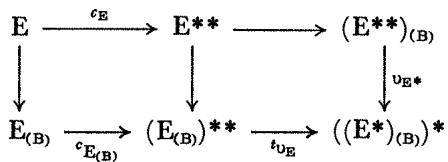
\includegraphics[keepaspectratio]{images/part003_7dd43288.jpg}}

is commutative.

\begin{enumerate}
\def\labelenumi{\arabic{enumi}.}
\setcounter{enumi}{4}
\item
  Let K be a field, A the product ring \(K^{N}\) , a the ideal \(K^{(N)}\) of A and B the ring A/a. Show that a is a projective A-module which is not finitely generated, although \(a_{(B)} = \{0\}\) .
\item
  With the rings A and B defined as in §1, Exercise 7, let M be an A-module; show that for M to be finitely generated (resp. free, projective), it is necessary and sufficient that \(M \otimes_{A} B\) be finitely generated (resp. free, projective).
\item
  Let \(\rho: A \to B\) be a ring homomorphism. For every left B-module \(F\) , define a canonical B-module homomorphism
\end{enumerate}

\[
\mathbf {F} \rightarrow \tilde {\rho} (\rho_ {*} (\mathbf {F}))
\]

and show that if E is a left A-module, the composite mappings

\[
\begin{array}{r l} & {\tilde {\rho} (\mathbf {E}) \to \tilde {\rho} (\rho_ {*} (\tilde {\rho} (\mathbf {E}))) \to \tilde {\rho} (\mathbf {E})} \\ & {\rho_ {*} (\mathbf {F}) \to \rho_ {*} (\tilde {\rho} (\rho_ {*} (\mathbf {F}))) \to \rho_ {*} (\mathbf {F})} \end{array}
\]

are the identity mappings.

\BourbakiExercisesSection

\begin{enumerate}
\def\labelenumi{\arabic{enumi}.}
\item
  Let \((\mathbf{E}_n, f_{nm})\) be the inverse system of \(\mathbf{Z}\) -modules whose indexing set is \(\mathbf{N}\) , such that \(\mathbf{E}_n = \mathbf{Z}\) for all \(n\) and, for \(n \leqslant m\) , \(f_{nm}\) is the mapping \(x \mapsto 3^{m - n}x\) . For all \(n\) , let \(u_n\) be the canonical mapping \(\mathbf{E}_n \to \mathbf{Z}/2\mathbf{Z}\) . Show that \((u_n)\) is an inverse system of surjective linear mappings but that \(\lim u_n\) is not surjective.
\item
  Let \((\mathbf{E}_{\alpha}, f_{\beta\alpha})\) be a direct system of A-modules. Show that the A-module \(\lim_{\rightarrow} E_{\alpha}\) is canonically isomorphic to the quotient of the direct sum \(\bigoplus_{\alpha} E_{\alpha} = F\) by the submodule N generated by the elements of the form \(j_{\beta}(f_{\beta\alpha}(x_{\alpha})) - j_{\alpha}(x_{\alpha})\) , for every ordered pair \((\alpha, \beta)\) such that \(\alpha \leqslant \beta\) and all \(x_{\alpha} \in E_{\alpha}\) , the \(j_{\alpha}: E_{\alpha} \to F\) being the canonical injections.
\item
  Let \((\mathbf{F}_n, f_{mn})\) be the direct system of \(\mathbf{Z}\) -modules such that \(\mathbf{F}_n\) is equal to \(\mathbf{U}_p\) ( \(\S 1\) , Exercise 12 (d)) for all \(n \geqslant 0\) and \(f_{mn}\) is the endomorphism \(x \mapsto p^{m-n}x\) of \(\mathbf{U}_p\) for \(n \leqslant m\) . Show that \(\lim_{\longrightarrow} \mathbf{F}_n = \{0\}\) although the \(f_{mn}\) are surjective.
\item
  Let \((\mathbf{F}_{\alpha}, f_{\beta \alpha})\) be a direct system of A-modules.
\end{enumerate}

\begin{enumerate}
\def\labelenumi{(\alph{enumi})}
\tightlist
\item
  For every A-module E, define a canonical Z-module homomorphism
\end{enumerate}

\[
\varepsilon : \varinjlim \operatorname{Hom} _ {\mathbf {A}} (\mathrm{E}, \mathrm{F} _ {\alpha}) \rightarrow \operatorname{Hom} _ {\mathbf {A}} (\mathrm{E}, \varinjlim \mathrm{F} _ {\alpha}).
\]

\begin{enumerate}
\def\labelenumi{(\alph{enumi})}
\setcounter{enumi}{1}
\item
  Show that if E is finitely generated, \(\varepsilon\) is injective. Give an example where \(\varepsilon\) is not injective (cf.~Exercise 3, taking \(E = \lim F_{\alpha}\) ).
\item
  Show that if E is finitely generated and the \(f_{\beta\alpha}\) are injective, \(\varepsilon\) is surjective. Give an example where \(E = \lim_{\longrightarrow} F_{\alpha}\) is free, the \(f_{\beta\alpha}\) are injective and \(\varepsilon\) is not surjective.
\item
  Show that if \(\mathbf{E}\) is projective and finitely generated, \(\varepsilon\) is bijective.
\end{enumerate}

\(^{*}(e)\) Let A be an integral domain and a an ideal of A which is not finitely generated. If \((a_{\alpha})\) is the family of finitely generated ideals contained in a, show that E = A/a is canonically isomorphic to the direct limit of the \(F_{\alpha} = A/a_{\alpha}\) , but that the homomorphism \(\varepsilon\) is not surjective.*
